\documentclass{article}
\usepackage{graphicx,amsmath}
\title{On the complexity of the square covering problem}
\author{\ldots}
\begin{document}
\maketitle
\begin{abstract}
We consider the problem of covering a set of points in the plane by 
using as few axis-aligned unit squares as possible, whose locations can be chosen freely. 
The problem is known to be NP-hard even in the case where the covering 
squares are chosen from a finite set. We propose an exact algorithm and a heuristic
in which the complexity can be controlled by narrowing the search space.
As the main contribution, we show how the complexity of the problem relates to the 
spatial density of nodes.
\end{abstract}
\section{Introduction}
We consider the problem of covering a set of points in the plane by 
using as few axis-aligned unit squares as possible, whose locations can be chosen freely. 
The problem is known to be NP-hard even in the case where the covering 
squares are chosen from a finite set. We propose an exact algorithm and a heuristic
in which the complexity can be controlled by narrowing the search space.
As the main contribution, we show how the complexity of the problem relates to the 
spatial density of nodes.

\subsection{Literature review}

\section{Algorithm}
The exact algorithm consists of two phases: In the first phase, we cover all \emph{corner nodes} 
and in the second phase, the remaining nodes are covered by enumerating the
possible solutions. The first phase runs in linear time and the complexity of the 
second phase is depends on the spatial density of nodes. For simplicity, unit squares 
are denoted by their lower left corners. The number of nodes is denoted by $n$.
\subsection{First phase}
The detection and covering of corner nodes is executed as follows: For each node $i \in \{1,\ldots,n\}$,
we check if there are non-covered nodes in the surrounding unit square sectors $A,B,C,D$, see Figure \ref{sectors01}. 
If all sectors are empty, node $i$ is covered by placing a square in any of the
sectors, for example $A$ (Figure \ref{sectors01}a). If exactly three of the sectors are empty, a square is placed in the fourth non-empty sector (Figure \ref{sectors01}b). 
In this case, the nodes in that sector are covered in addition to node $i$.
If the number of empty sectors is less than three (Figure \ref{sectors01}c), no square is placed and 
the algorithm proceeds to the next node.
In the first two cases, we say that the node $i$ is a corner node.

\begin{figure}[ht]
\begin{center}
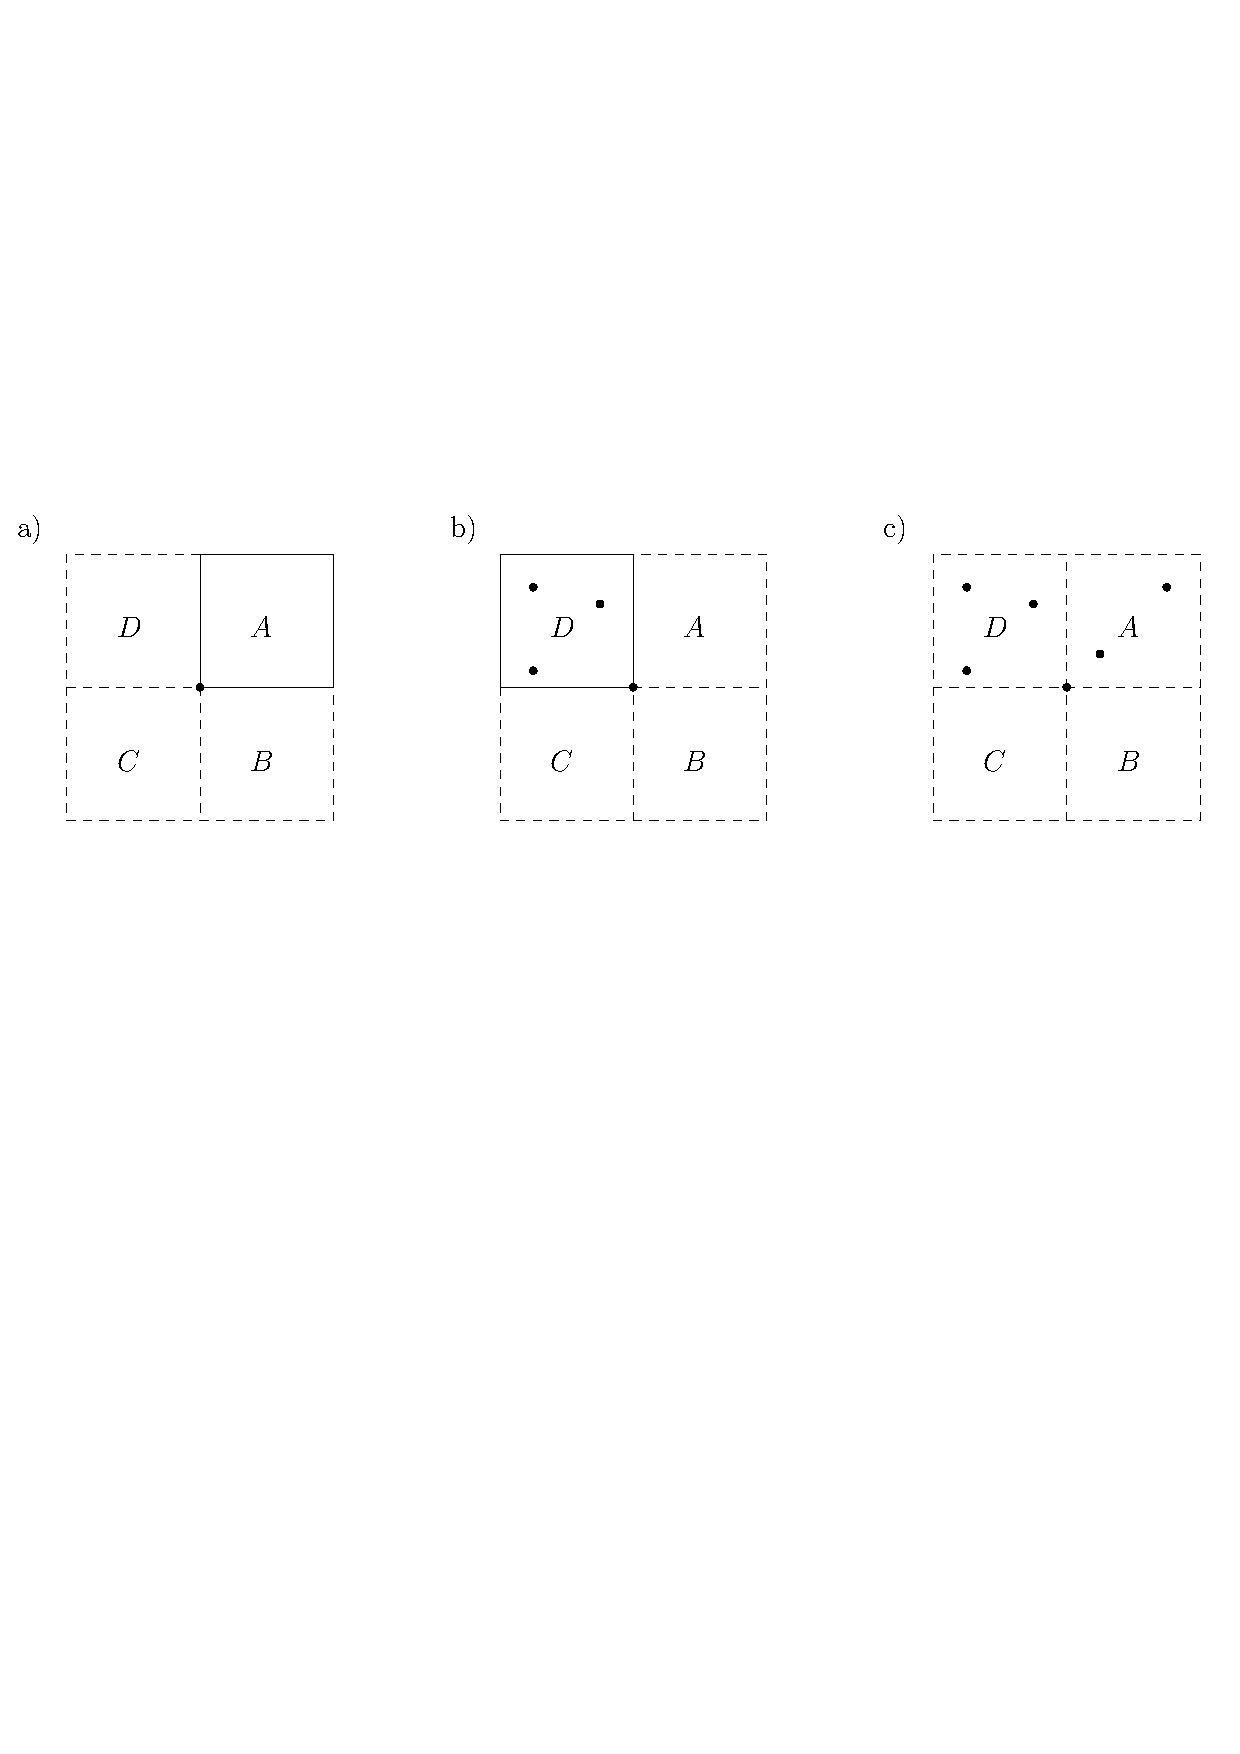
\includegraphics[width=0.9\columnwidth]{sectors01}
\caption{The detection of corner nodes. Figure a shows the four surrounding
sectors of node $i$, denoted by $A,B,C,D$. In Figure b, the three sectors $A,B,C$
are empty and thus $i$ is a corner node and a square is placed at sector $D$.}
\label{sectors01}
\end{center}
\end{figure}


The first phase is repeated until all corner nodes are covered. Note that 
covering a corner node may generate new corner nodes.

\subsection{Second phase}
The second phase is executed as follows: Let $(x_m,y_m)$ be an uncovered node for which
the $y$-coordinate is minimized, that is, $y_m \leq y_i$ for all $i \in \{1,\ldots,n\}$.
Since the node $(x_m,y_m)$ is not a corner node, we know that sectors $D$ and $A$ are both non-empty 
(see Figure \ref{sectors01}). We denote the nodes in sector $D$ by 
$(x_1,y_1),\ldots,(x_{m},y_{m})$, sorted in ascending order of the $x$-coordinate. 
If there are several nodes with equal $x$-coordinates, these nodes are considered as a single node.

First, a \emph{set of nondominated squares} $Q$ is formed. By nondominated we mean 
that $C_q \not \subset C_{q'}$ for all $q,q' \in Q$, where $C_q$ and $C_{q'}$ denote
the sets of nodes covered by squares $q$ and $q'$, respectively. The nondominated 
set is found as follows: 1. Add a square $q_1 = (x_1,y')$ to $Q$. 2. For $i = 2,3,\ldots,m$,
let $C_{q_i}$ denote the set of nodes covered by the square $q_i = (x_i^D,y')$. If $C_{q_i} \not \subset C_{q_{i-1}}$,
add $q_{i}$ to $Q$.

\begin{figure}[ht]
\begin{center}
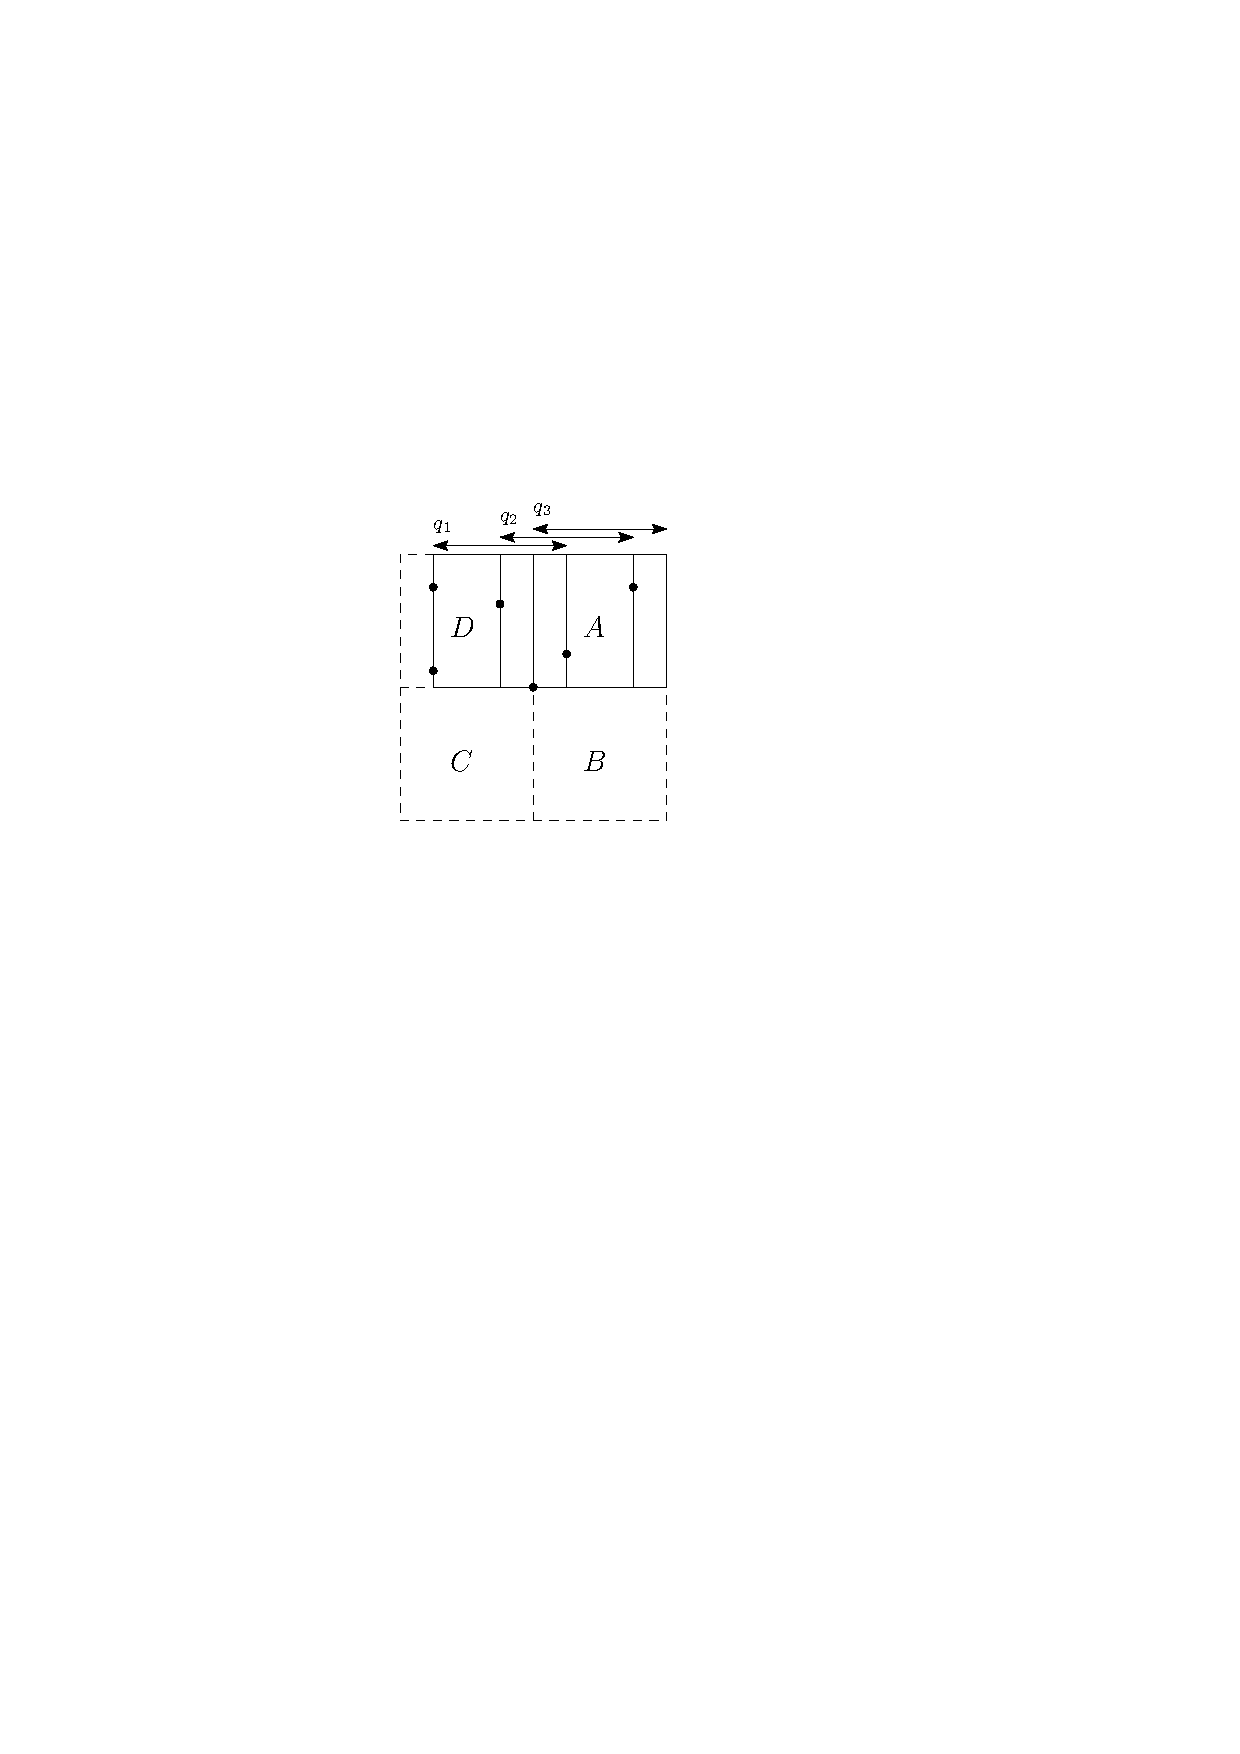
\includegraphics[width=0.4\columnwidth]{nondominated01}
\caption{The nondominated set $Q$. We consider the squares $q_1,q_2,q_3$ placed at
the $x$-coordinates of the points in sector $D$. The squares $q_1$ and $q_2$ are included in 
the nondominated set, since all nodes covered by $q_2$ are not covered by $q_1$, that is, $C_{q_2} \not \subset C_{q_1}$.
However, $q_3$ is not included in the nondominated set since $C_{q_3} \subset C_{q_2}$.
}
\label{nondominated01}
\end{center}
\end{figure}

The algorithm proceeds recursively as follows: For each $q \in Q$, a square is placed at $q$, 
the nodes inside $q$ are covered and the second phase is repeated.

Executing the second phase may produce several different solutions to the problem since all
squares in the nondominated set are considered each time the second phase is executed.
The optimal solution to the problem is obtained by choosing the solution in which the 
number of squares is minimized.


\subsection{Heuristic}
The exact solution is naturally extended to a heuristic by narrowing
the dominating set of squares at each step to a certain maximum number $M$
of squares. The narrowed set $Q'$ is determined by including the squares 
$q_i \in Q$ that cover the most nodes. If $M=1$, the algorithm runs in linear time.
In order to control the computational effort smoothly, $M$ can be defined
as a random variable, for example, $M=1$ with probability $p$ and $M=2$ with probability $p-1$.


\section{Complexity analysis}
The general set cover problem is known to be NP-hard. In this work we focus on the
average-case complexity of the exact algorithm as a function of the point
density $\lambda$. 
Suppose that the number of nodes $\xi(V)$ in a region of size $V$ follows the Poisson 
distribution, that is, 
\begin{align*}
P(\xi(V)=k) = \frac{(\lambda V)^k}{k!} e^{-\lambda V},
\end{align*}
where $\lambda$ is the point density of nodes in a region of unit size.

\subsection{First phase}
A node $i$ is a corner node with probability 
\begin{align}
\notag
P_c & =4 \cdot P(\xi(3)=0) \cdot P(\xi(1) > 0) + P(\xi(4)=0) \\ 
\label{cornerprob}
& = 4 e^{-3 \lambda} (1-e^{-\lambda}) + e^{-4 \lambda} = e^{-4 \lambda } (4 e^{\lambda }-3).
\end{align}
Note that in finite regions, the probability is greater due to border effects. In addition,
the elimination of corner nodes may generate new corner nodes. 
Thus, the probability \eqref{cornerprob} gives us a lower bound 
$nP_c$ for the expected number of corner nodes. 
The corresponding expected number of nodes covered by the squares 
covering the corner nodes equals $(\lambda + 1) n P_c$.

\subsection{Second phase}
The expected number of nodes remaining in the second phase is bounded
by $n(1-(\lambda + 1)P_c)$. At each step, the expected number of nodes 
in sector $D$ (including the center node) equals $\lambda + 1$, which is
an upper bound for the expected number of squares $q$ in the nondominated set $Q$.

Each square in the nondominated set covers on average $\lambda + 1$ nodes and thus the
expected number of steps needed in the second phase to cover all nodes is bounded by 
$n(1-(\lambda + 1)P_c) / (\lambda + 1)$. Since the expected number of branches beginning at 
each step is $\lambda + 1$, the average-case complexity of the exact solution is given by
\begin{align*}
(\lambda + 1)^{n(\frac{1}{\lambda + 1} - P_c)} = 
(\lambda+1)^{n(\frac{1}{\lambda + 1} - e^{-4 \lambda } (4 e^{\lambda }-3))}.
\end{align*}
The factor of $n$ is maximized ($\approx 0.371$) at $\lambda \approx 1.26$. Thus the average case 
complexity is of order $\mathcal{O}((\lambda+1)^{0.371 n})$.
%\begin{align*}
%-4 e^{-3 \lambda }+4 e^{-4 \lambda } \left(-3+4 e^{\lambda }\right)-\frac{1}{(1+\lambda )^2} = 0 \\
%\end{align*}


\section{Conclusions}
We have considered the average-case complexity of the square covering problem 
as a function of the spatial density $\lambda$ of nodes.
We suggest a two-phase exact solution and show that the expected complexity 
is of order $\mathcal{O}((\lambda+1)^{0.371 n})$.
By narrowing the search space, the exact method is extended to an adjustable 
heuristic in which the computational effort can be controlled smoothly. The 
simplest version of the heuristic runs in linear time.

\end{document}